% mn2esample.tex
%
% v2.1 released 22nd May 2002 (G. Hutton)
%
% The mnsample.tex file has been amended to highlight
% the proper use of LaTeX2e code with the class file
% and using natbib cross-referencing. These changes
% do not reflect the original paper by A. V. Raveendran.
%
% Previous versions of this sample document were
% compatible with the LaTeX 2.09 style file mn.sty
% v1.2 released 5th September 1994 (M. Reed)
% v1.1 released 18th July 1994
% v1.0 released 28th January 1994

\documentclass[useAMS,usenatbib]{mn2e}
\usepackage{graphicx,subfigure}
\usepackage{amsmath}
\usepackage{rotating}
\usepackage{color}
\usepackage{times}

%\author[dd]{dd}
\begin{document}
\def \apj {ApJ}
\def \apss {Ap{\&}SS}
\def \mnras {MNRAS}
\def \aj {AJ}
\def \araa {ARA\&A}
\def \aapr {A\&ARv}
\def \pasa {PASA}
\def \aap {AAP}
\def \aaps {AAPS}
\def \apjl {ApJL}
\def \apjs {ApJS}
\def \pasj {PASJ}
\def \nat {Nature}
% remove the useAMS option.
%
% useAMS allows you to obtain upright Greek characters.
% e.g. \umu, \upi etc.  See the section on "Upright Greek characters" in
% this guide for further information.
%
% If you are using AMS 2.0 fonts, bold math letters/symbols are available
% at a larger range of sizes for NFSS release 1 and 2 (using \boldmath or
% preferably \bmath).
%
% The usenatbib command allows the use of Patrick Daly's natbib.sty for
% cross-referencing.
%
% If you wish to typeset the paper in Times font (if you do not have the
% PostScript Type 1 Computer Modern fonts you will need to do this to get
% smoother fonts in a PDF file) then uncomment the next line
% \usepackage{Times}

%%%%% AUTHORS - PLACE YOUR OWN MACROS HERE %%%%%

\newcommand{\kpc}{{\rm\,kpc}}
\newcommand{\mpc}{{\rm\,Mpc}}
\newcommand{\pc}{{\rm\,pc}}
\newcommand{\kms}{{\rm\,km\,s^{-1} }}
\newcommand{\msun}{{\rm\,M_\odot }}
\newcommand{\lsun}{{\rm\,L_\odot }}
\newcommand{\rsun}{{\rm\,R_\odot}}
\newcommand{\ngcs}{NGC~147 }
\newcommand{\ngcf}{NGC~185 }
%\newcommand{\deg}{^\circ}

\newcommand{\km}{{\rm\,km}}
\newcommand{\cm}{{\rm\,cm}}
\newcommand{\yr}{{\rm\,yr}}
\newcommand{\au}{{\rm\,AU}}
\newcommand{\g}{{\rm\,g}}
%***************\newcommand{\om}{\Omega_0}
%***************\newcommand{ \ca} {{\it ca.\/}}
%***************%\newcommand{ \r} {r$^{1/4}$ }
%***************\newcommand{ \magnitude} {$^{\rm m}$}
%***************\newcommand{\kr}{${\cal K}_r$}
%***************\newcommand{\kz}{${\cal K}_z$}
%***************\newcommand{\kzz}{${\cal K}_z(z)$}
%***************\newcommand{\mss}{{\rm M}_\odot \rm pc^{-2}}
%***************\newcommand{\msss}{{\rm M}_\odot \rm pc^{-3}}
%***************\newcommand{\fmmm}[1]{\mbox{$#1$}}
%***************\newcommand{\scnd}{\mbox{\fmmm{''}\hskip-0.3em .}}
%***************\newcommand{\scnp}{\mbox{\fmmm{''}}}
%***************\newcommand{\mcnd}{\mbox{\fmmm{'}\hskip-0.3em .}}
\newcommand{\Aa}{\; \buildrel \circ \over {\rm A}}
%***************%\newcommand{\AA}{$\; \buildrel \circ \over {\rm A}$}
%***************
%***************% MISCELLANEOUS:
%***************% angles in degrees
%***************%\degg produces degree symbol so that 3\sec5 produces 3.`5 with the degree
%***************%symbol and the period aligned.
%***************\newcommand{\degg}{\hbox{$\null^\circ$\hskip-3pt .}}
%***************%\sec produces arcsec symbol so that 3\sec5 produces 3."5 with the second
%***************%symbol and the period aligned.
%***************%\newcommand{\sec}{\hbox{"\hskip-3pt .}}
%***************\newcommand{\half}{{\scriptstyle{1\over2}}}
%***************%\s produces tilde in mathmode or horizontal mode.
%***************\newcommand{\s}{\ifmmode \widetilde \else \~\fi}
%***************%\newcommand{\=}{\overline}
%***************\newcommand{\scre}{{\cal E}}
%***************%\newcommand{\spose#1{\hbox to 0pt{#1\hss}}
%***************\newcommand{\larrow}{\leftarrow}
%***************\newcommand{\rarrow}{\rightarrow}
%***************\newcommand{\llangle}{\langle\langle}
%***************\newcommand{\rrangle}{\rangle\rangle}
%***************\newcommand{\etal}{{\it et al.\ }}
%***************\newcommand{\cf}{{\it cf.\ }}
%***************\newcommand{\eg}{{e.g.,\ }}
%***************\newcommand{\ie}{{i.e.,\ }}
%***************%\lta and \gta produce > and < signs with twiddle underneath
%***************\newcommand{\lta}{\mathrel{\spose{\lower 3pt\hbox{$\mathchar"218$}}
%***************     \raise 2.0pt\hbox{$\mathchar"13C$}}}
%***************\newcommand{\gta}{\mathrel{\spose{\lower 3pt\hbox{$\mathchar"218$}}
%***************     \raise 2.0pt\hbox{$\mathchar"13E$}}}
%***************%\Dt and \dt put Newton's notation dots above upper and lower case chars
%***************\newcommand{\Dt}{\spose{\raise 1.5ex\hbox{\hskip3pt$\mathchar"201$}}}    % upper case
%***************\newcommand{\dt}{\spose{\raise 1.0ex\hbox{\hskip2pt$\mathchar"201$}}}    % lower case
%***************\newcommand{\del}{\nabla}
%***************\newcommand{\delv}{\bb\nabla}
%***************%\newcommand{\r}{${\rm r^{1/4}}$}
%***************
%***************\newcommand{\jla}{J_{\lambda}}
%***************\newcommand{\jmu}{J_{\mu}}
%***************\newcommand{\jnu}{J_{\nu}}
%***************\newcommand{\pomega}{\varpi}
%***************\newcommand{\sigla}{\sigma_{\lambda}}
%***************\newcommand{\sigmu}{\sigma_{\mu}}
%***************\newcommand{\signu}{\sigma_{\nu}}
%***************\newcommand{\dotsfill}{\leaders\hbox to 1em{\hss.\hss}\hfill}
%***************%\newcommand{\sun}{\odot}
%***************%\newcommand{\earth}{\oplus}
%***************
%***************\newcommand{\Gyr}{{\rm\,Gyr}}
%***************\newcommand{\FeH}{{\rm[Fe/H]}}
%***************\newcommand{\kmsd}{{\rm\,km/s/degree}}
%***************
%***************\newcommand{\ud}{\mathrm{d}}
%***************
%***************\newcommand{\ngcs}{NGC~147}
%***************\newcommand{\ngcf}{NGC~185}
%***************
%%%%%%%%%%%%%%%%%%%%%%%%%%%%%%%%%%%%%%%%%%%%%%%%

\title[The Andromeda plane]{The Andromeda Plane}
\author[Arias et al.]{
{\parbox{\textwidth}{
Veronica Arias$^{1}$\thanks{E-mail:v.arias@uniandes.edu.co}, 
Magda Guglielmo$^2$,
Geraint F. Lewis$^2$, 
%Nicholas F. Bate$^$,
%Anthony Conn$^2$,
%Rodrigo A. Ibata$^3$,
%Nuwanthika Fernando$^2$, 
%Alan W. McConnachie$^3$, 
%Nicolas Martin$^{5,6}$, 
et~al.\\}}
\vspace{0.1cm}\\
\parbox{\textwidth}{
$^1$Departamento de F\'isica, Universidad de los Andes, Cra. 1 No. 18A-10, Edificio Ip, Bogot\'a, Colombia\\
$^2$Sydney Institute for Astronomy, School of Physics, A28, The University of Sydney, NSW 2006, Australia \\
%$^3$Observatoire de Strasbourg, 11, rue de l'Universit\'e, F-67000, Strasbourg, France\\
%$^4$NRC Herzberg Institute for Astrophysics, 5071 West Saanich Road, Victoria, British Columbia, Canada, V9E 2E7 \\
%$^5$Institute for Astronomy, University of Edinburgh, Royal Observatory, Blackford Hill, Edinburgh, EH9 3HJ, U.K. \\
%$^6$Max-Planck-Institut für Astronomie, Königstuhl 17, D-69117 Heidelberg, Germany\\
}}

\date{Accepted xxx. Received xxxx; in original form xxxx}

\pagerange{\pageref{firstpage}--\pageref{lastpage}} \pubyear{2002}

\maketitle

\label{firstpage}

\begin{abstract}

\end{abstract}

\begin{keywords}
%galaxies -- XXX -- XXX 
Local Group --- galaxies: dwarf -- galaxies: individual (M31)  
\end{keywords}

\section{Introduction}

The anysothropic distribution of the satellite galaxies in the Milky
way has been long known (Linden-Bell, Pawlowsky).

Plane of satellites in M31 (Conn, Ibata). 14kpc, extended 400 kpc.
Corrotating.
   
Other evidence of planes in XXX(Tully) and evidence of corrotation in
SDSS (Ibata).

First attempts to find such planar structures in only DM simulations
(Baumgardt 2013) found a probablility of XXX but these numbers
decreased even further to XXXX in two revised studies by Ibata 2013
and Pawlowsky 2013, who concluded that the observed structures cannot
be explained by $\Lambda$CDM DM only simulations.

In recent papers Sawala 2014 finds that when including baryonic matter in
cosmological simulations the discrepancies in the number and
distribution of satellites between simulations and
observations disapear.
 
Additionally, Gillet 2015, finds corrotating
planes in simulations that include hydrodynamics and concludes that the M31
plane could be the result of a group of satellites that entered their
host together and have coherent orbits and some satellites that are on
the plane incidentaly and probably have significant velocities
perpendicular to the plane. 

This work seems to reconcile the results
from simulations with the observations, with the caveat that the plane observed in the 
Andromeda galaxy is always colder than the planes found in simulations, 
and hints at possible formation scenarios for the M31 plane.  

Formation scenarios have also been explored by Libeskind XXX, who
showed that, in the simulations, there were preferential directions
for satellite accretion dictated by the filamentary structure of the
cosmic web and in particular the velocity shear vector.  

This result
was observationaly tested by Tempel 2015 and XXXXXXXX using the SDSS
catalog to reconstruct the filamentary structure XXXXX.

Buck et al. 

Other possible explanations for the alignement of the satellites have
been proposed by Kroupa et al 20XX and Pawlowski 20XX who claim that
the satellites of the MW and of M31 are tidal dwarfs. 

This scenario
has also been explored by Fouquet (XXXXX) who finds, using N-Body
simulations, that the satellites of the Milky Way and M31 could be the
result of a past interaction between these two galaxies. 

%Another
%scenario, proposed by Goerdt 2013, proposes that the plane satellites
%were delivered by cold gas streams.

This paper is organised as follows. 
In Section \ref{Method} we describe introduce the numerical model used to describe both the Milky Way and the M31 potentials and the restriction we impose on the unknown tangential velocities of the satellites. We the show in Section XXXX, the resulting orbits that we obtain. Finally, we discuss the posible implications of XXXXXXXX   

%%%%%\section{Numerical Model}\label{secNumMod}
%%%%%In this paper, we study the dynamics of the satellite galaxies of Andromeda. We integrate the orbits of the individual satellites both backwards and forwards in time and use a point mass approximation for the satellites and rigid potentials for Andromeda and for the Milky Way. 
%%%%%
%%%%%To describe the Andromeda potential we use a three component model first proposed by \cite{2006MNRAS.366..996G}.  
%%%%%With a Navarro-Frenk and White (NFW) dark matter halo potential \citep{1997ApJ...490..493N} given by
%%%%%\begin{equation}
%%%%%\Phi_{\rm{halo}}(r)=-\frac{\rm{GM_{\rm{halo}}}}{r}\log \left(\frac{r}{r_{\rm{halo}}}+1\right),
%%%%%\label{NFW}
%%%%%\end{equation}   
%%%%%An exponential disk given by
%%%%%\begin{equation}
%%%%%\Phi_{\rm{disk}}(r)=-2{\pi}G\Sigma_{0}{r_{\rm{disk}}}^2\left[\frac{1-\exp^{-r/r_{\rm{disk}}}}{r}\right]
%%%%%\end{equation}   
%%%%%and a Hernquist profile for the bulge\citep{1990ApJ...356..359H}
%%%%%\begin{equation}
%%%%%\Phi_{\rm{bulge}}(r)=-\frac{\rm{GM_{{bulge}}}}{r_{\rm{bulge}}+r}\mbox{.}
%%%%%\label{Hernquist}
%%%%%\end{equation}\\
%%%%%
%%%%%For Milky Way potential we use also a Hernquist bulge, a NFW halo potential (equations (\ref{Hernquist}) and (\ref{NFW})), 
%%%%%and a Miyamoto-Nagai potential \citep{1975PASJ...27..533M} for the disk, given by
%%%%%\begin{equation}
%%%%%\Phi_{\rm{disk}}(R,z)=-\frac{\rm{GM_{disk}}}{\left(R^2+\left(r_{\rm{disk}}+{\sqrt{(z^2+b^2)}}\right)^2\right)^{1/2}}
%%%%%\end{equation}\\
%%%%%
%%%%%The parameters are listed in Table \ref{tabPot}.
%%%%%%The models described above for M31 and the Milky Way are kept the same in all the different steps our analysis. 
%%%%%%In the case of the N-body simulation, (see Section \ref{secNbody}), the Gadget-2 code \citep{2005MNRAS.364.1105S} has been modified in order to include M31 and the Milky Way as rigid potentials.
%%%%%
%%%%%%{\color{blue} Additionally, for all the dynamical analysis, we use a coordinate system centred in M31 and for which M31's disk lies in the $xy$ plane. 
%%%%%%The distances, right ascensions and declinations of the satellites 
%%%%%%are transformed into this coordinate system as described by \cite{2012ApJ...758...11C}.
%%%%%%The measured velocities of the satellites are also transformed into this coordinate system by subtracting M31's heliocentric velocity from the z-component of the satellites heliocentric velocities \citep{2013ApJ...768..172C}.} 
%%%%%
%%%%%\begin{table}
%%%%%\centering
%%%%%\begin{tabular}{l l }
%%%%%\multicolumn{2}{c}{\textbf{M31}}\\
%%%%%\hline
%%%%%\hline
%%%%%$\rm{M}_{bulge}$   	& $2.86\times{10^{10}}\,\rm{M}_{\odot}$\\
%%%%%$\rm{r}_{bulge}$	& $0.61\,\rm{kpc}$\\
%%%%%$\rm{M}_{disk}$		&  $8.4\times{10^{10}}\,\rm{M}_{\odot}$\\
%%%%%$\rm{r}_{disk}$		& $5.4\,\rm{kpc}$\\
%%%%%$\Sigma_{0}$		& $4.6\times10^{8}\,\rm{M}_{\odot}\rm{kpc^{-2}}$\\
%%%%%$\rm{M}_{halo}$		&  $103.7\times{10^{10}}\,\rm{M}_{\odot}$\\
%%%%%$\rm{r}_{halo}$		& $13.5\,\rm{kpc}$\\
%%%%%&\\
%%%%%\multicolumn{2}{c}{\textbf{MW}}\\
%%%%%\hline
%%%%%\hline
%%%%%$\rm{M}_{bulge}$       & $ 3.4\times{10^{10}}\,\rm{M}_{\odot}$   \\
%%%%%$\rm{r}_{bulge}$       & $ 0.7\,\rm{kpc}$                        \\
%%%%%$\rm{M}_{disk}$        & $ 10.0\times{10^{10}}\,\rm{M}_{\odot}$  \\
%%%%%$\rm{r}_{disk}$        & $ 6.65\,\rm{kpc}$                       \\
%%%%%$\rm{b} $              & $ 0.26\,\rm{kpc}$                       \\
%%%%%$\rm{M}_{halo}$        & $ 91.36\times{10^{10}}\,\rm{M}_{\odot}$   \\
%%%%%$\rm{r}_{halo}$        & $ 24.54\,\rm{kpc}$                        \\
%%%%%$\rm{d}_{\rm{M31-MW}}$ & $ 779\,\rm{kpc}$                        \\   
%%%%%\hline
%%%%%\hline
%%%%%\end{tabular}
%%%%%\caption{List of parameters used for M31 \protect\cite{2006MNRAS.366..996G} and the Milky Way potentials \protect\cite{2005ApJ...635..931B}.}
%%%%%\label{tabPot}
%%%%%\end{table}
%%%%%
\section{Method}
\label{Method}
\subsection{M31 coordinate system}
%We use the distances and positions 
We have the observed line of sight velocities and distances and positions of the satellites. 
We transform those to a coordinate system centered in M31 and whose xxxx-axis point in the M31-MW direction as shown in figure XXXX.
The new x, y and z positions are given by (Conn et al 2013) (Arias et al 2015)\citep{2013ApJ...766..120C,2013Natur.493...62I}

\begin{equation}
x =
\end{equation}\\
\begin{equation}
y =
\end{equation}\\
\begin{equation}
z =
\end{equation}\\

We use a similar principle for the velocities 

\begin{equation}
V_x =
\end{equation}\\
\begin{equation}
V_y =
\end{equation}\\
\begin{equation}
V_z =
\end{equation}\\

Finally, we rotate this coordinate system so that the xy plane coincides with M31's disk.  

\subsection{Potentials of M31 and the Milky Way}
The Andromeda potential is described as a three component model, first proposed by \cite{2006MNRAS.366..996G}.  
The dark matter halo is described as a Navarro-Frenk and White (NFW) potential \citep{1997ApJ...490..493N} given by
\begin{equation}
\Phi_{\rm{halo}}(r)=-\frac{\rm{GM_{\rm{halo}}}}{r}\log \left(\frac{r}{r_{\rm{halo}}}+1\right),
\label{NFW}
\end{equation}   
The disk component of the potential is given by
\begin{equation}
\Phi_{\rm{disk}}(r)=-2{\pi}G\Sigma_{0}{r_{\rm{disk}}}^2\left[\frac{1-\exp^{-r/r_{\rm{disk}}}}{r}\right]
\end{equation}   
and the bulge component follows a Hernquist profile \citep{1990ApJ...356..359H}
\begin{equation}
\Phi_{\rm{bulge}}(r)=-\frac{\rm{GM_{{bulge}}}}{r_{\rm{bulge}}+r}\mbox{.}
\label{Hernquist}
\end{equation}\\

The Milky Way potential is described by a Hernquist bulge, a NFW halo potential (see equations (\ref{Hernquist}) and (\ref{NFW})), 
and a Galactic disk described by a Miyamoto-Nagai potential \citep{1975PASJ...27..533M} given by
\begin{equation}
\Phi_{\rm{disk}}(R,z)=-\frac{\rm{GM_{disk}}}{\left(R^2+\left(r_{\rm{disk}}+{\sqrt{(z^2+b^2)}}\right)^2\right)^{1/2}}
\end{equation}\\


\subsection{Velocities in the tangential plane}
Collins et al. and Tollerud et al. measured the line of sight (or radial velocities) of XXX of M31's satellite galaxies but we lack information on their proper motions.  
In this work we investigate the possible orbits of the satellites in M31's potential and therefore we need to account for the unknown proper motions. 
We make the following assumption: if the plane of satellites is a
dynamicaly coherent structure, then the total velocities of the
satellites must be contained in such plane. We have measured radial
velocities $v_r$ (Collins 2013, SPLASH survey 20XX) so we can construct a
tangential velocity vector such that the total velocity is on the
plane. This asumption determines the direction of the unknown tangential
velocity vector and we are left with only its magnitude as a free
parameter. If we vary this parameter between reasonable values
(-$\sqrt 3 v_r$ + $\sqrt 3 v_r$) 



\section{Results}
\label{Results}
\begin{figure}
\centering
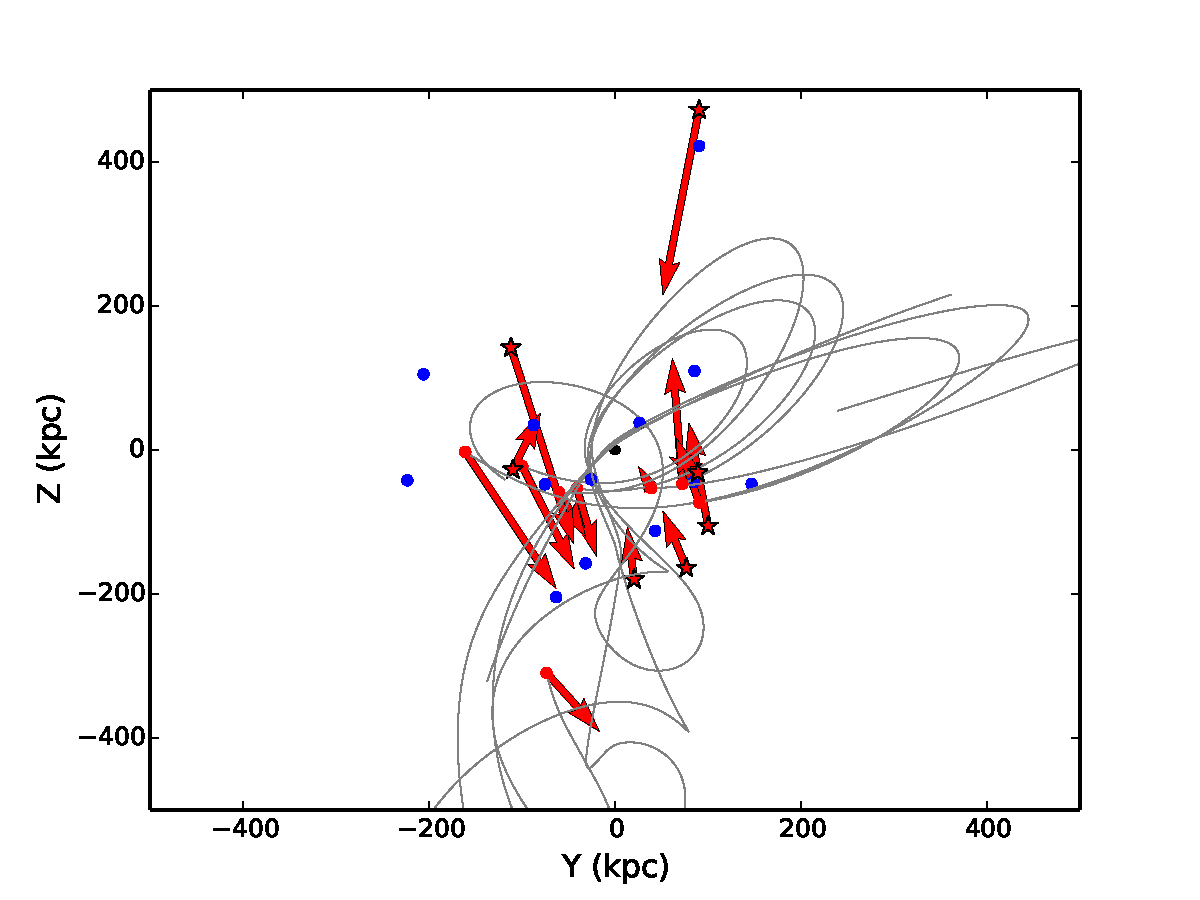
\includegraphics[width=\hsize]{SnapshotSatellites_All_BeforeRotationM300_yz_All_Fwd_NSIMW_3000.pdf}\\
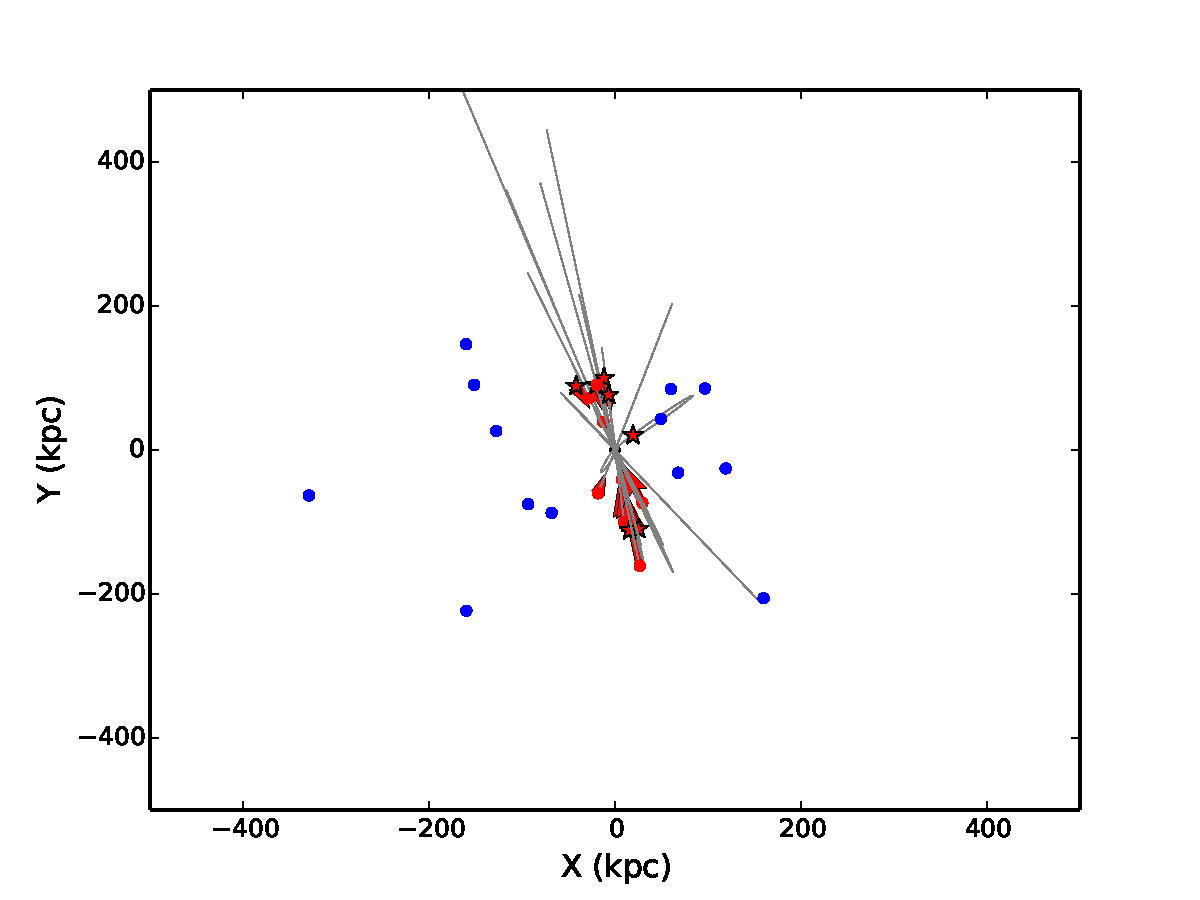
\includegraphics[width=0.5\hsize]{SnapshotSatellites_All_BeforeRotationM300_xy_All_Fwd_NSIMW_3000.pdf}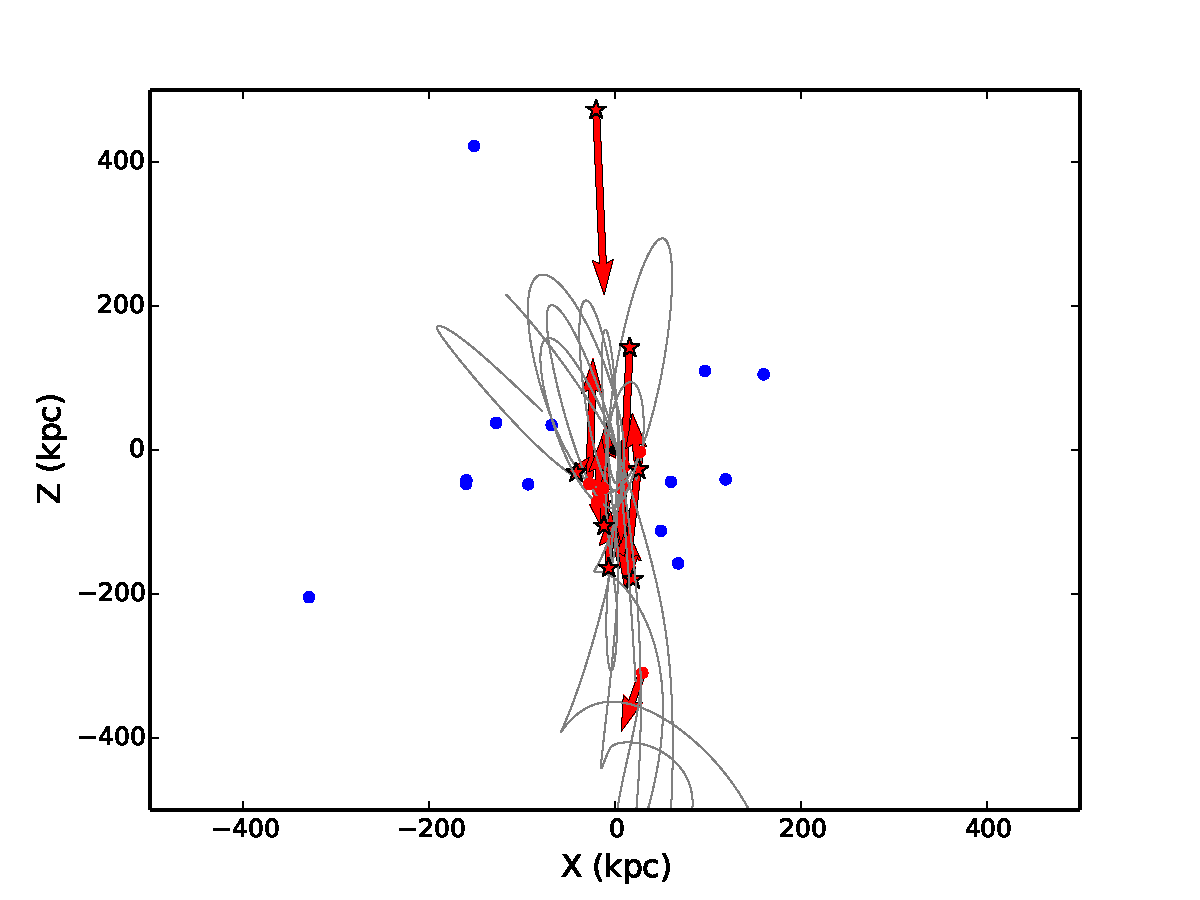
\includegraphics[width=0.5\hsize]{SnapshotSatellites_All_BeforeRotationM300_xz_All_Fwd_NSIMW_3000.pdf}\\
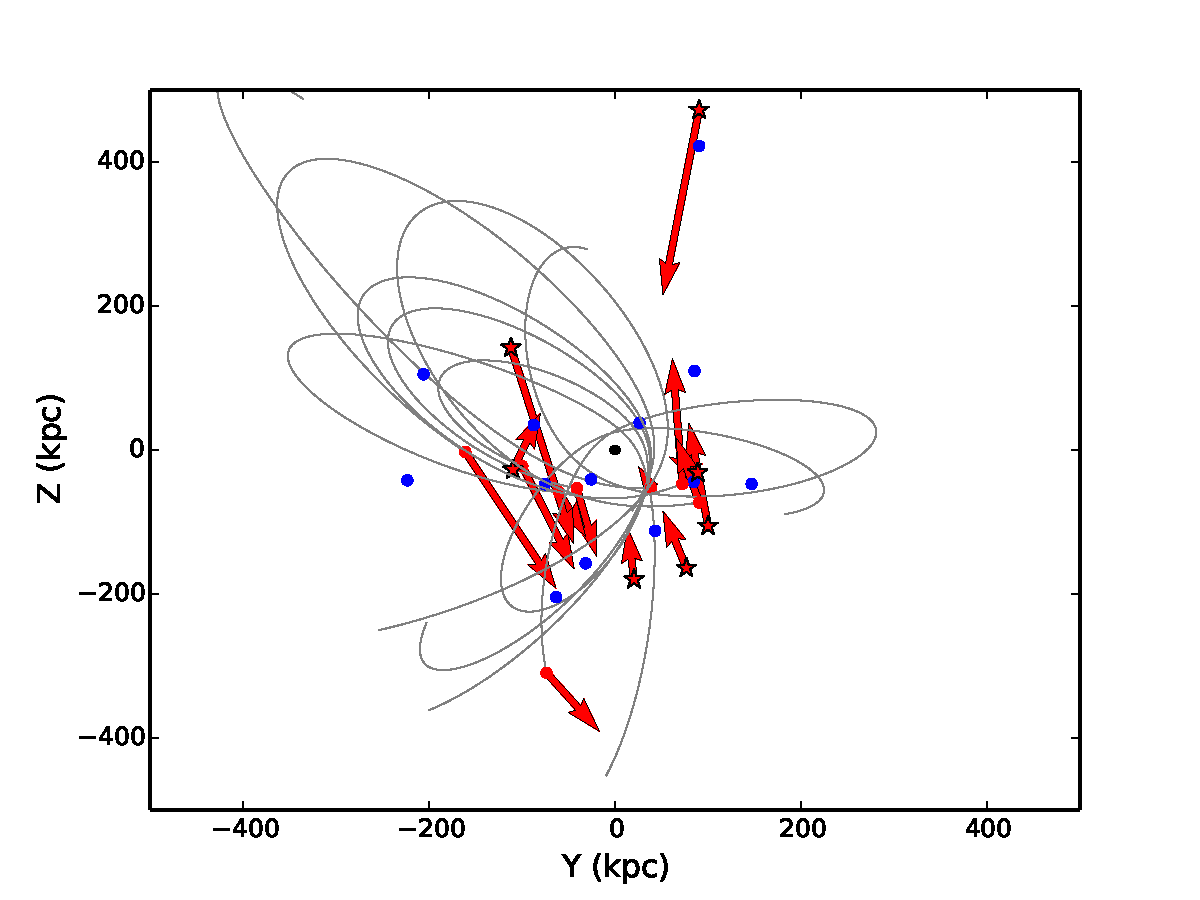
\includegraphics[width=\hsize]{SnapshotSatellites_All_BeforeRotationM300_yz_All_Bwd_NSIMW_3000.pdf}\\
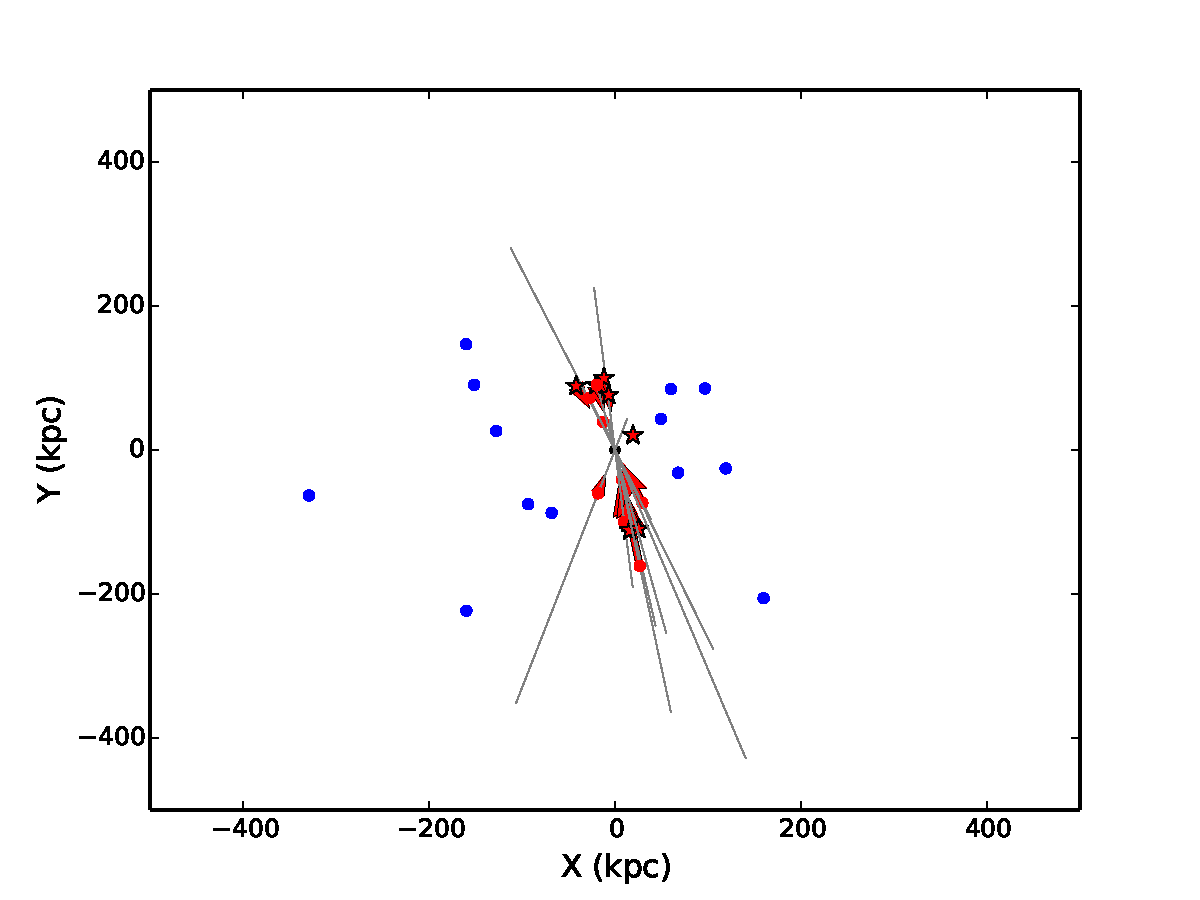
\includegraphics[width=0.5\hsize]{SnapshotSatellites_All_BeforeRotationM300_xy_All_Bwd_NSIMW_3000.pdf}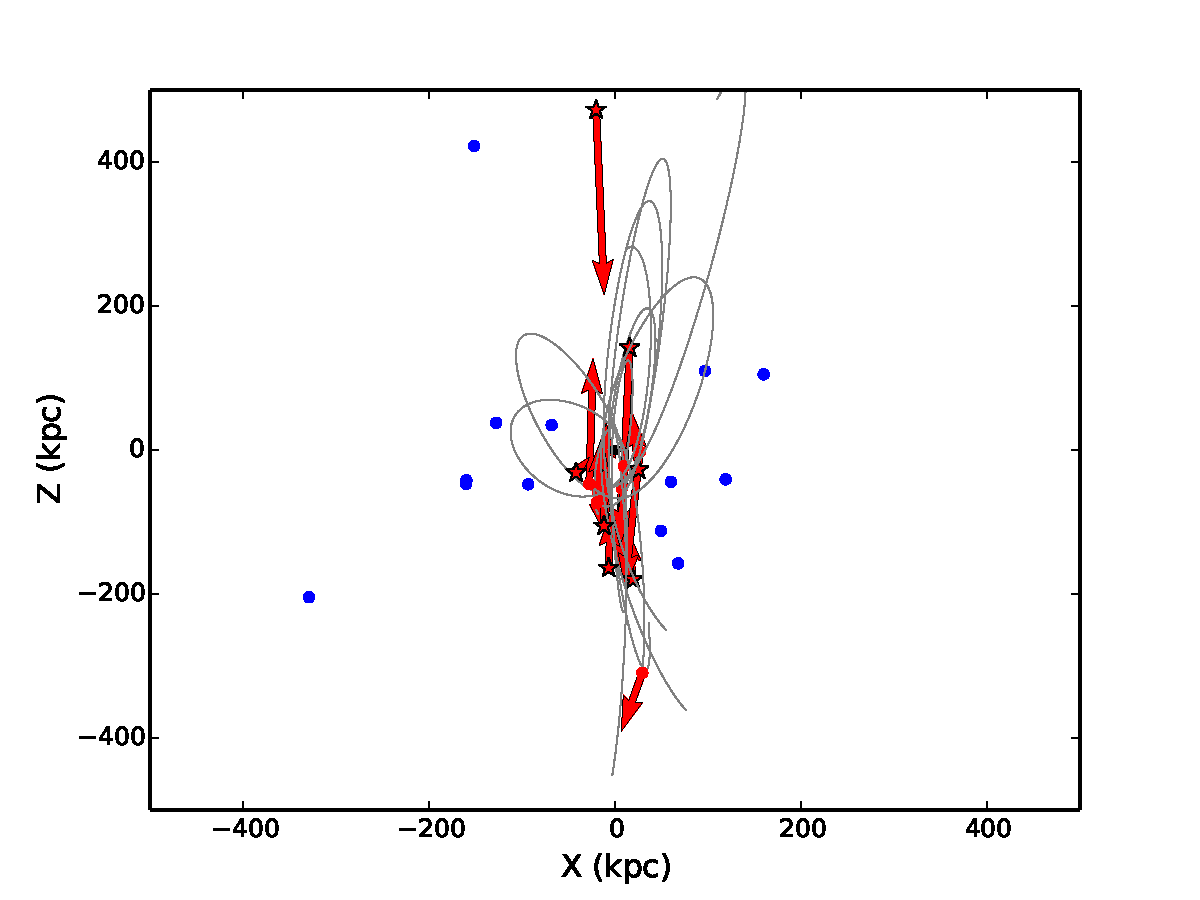
\includegraphics[width=0.5\hsize]{SnapshotSatellites_All_BeforeRotationM300_xz_All_Bwd_NSIMW_3000.pdf}\\
\caption{.}
\label{fig:StreamPlaneOrbit}
\end{figure}

\begin{figure}
\centering
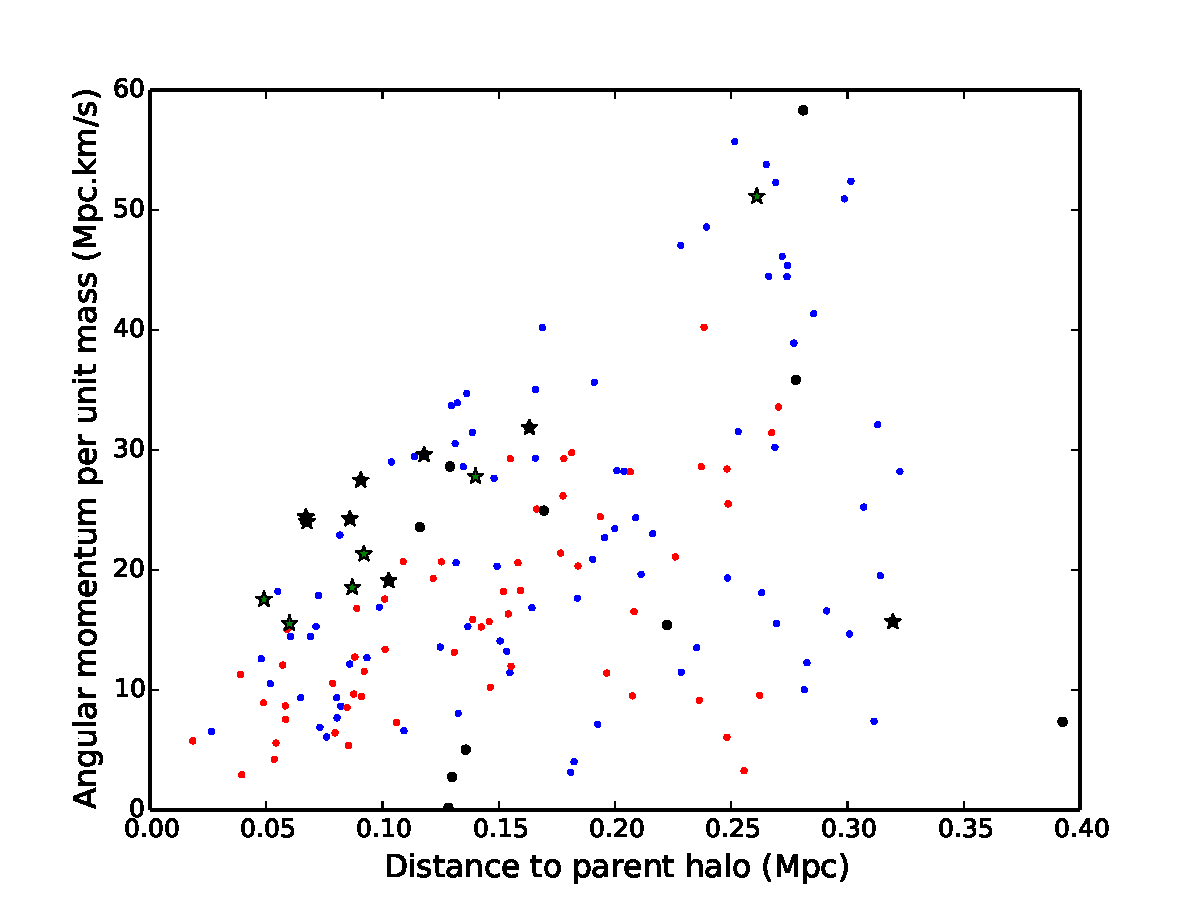
\includegraphics[width=\hsize]{Halo_pos_LRomulusRemus.pdf}\\
\end{figure}
\section{Discussion} 
\section{Acknowledgements}
%M. G. acknowledges the Australia Postgraduate Award (APA) for supporting her PhD candidature and the Astronomical Society of Australia for its travel support. 
%N. F. acknowledges the Dean's International Post Graduate Scholarship of the Faculty of Science, University of Sydney.
\bibliographystyle{mn2e}
\bibliography{Dwarfs}



\label{lastpage}

\end{document}
